\documentclass[11pt]{article}
\usepackage{geometry,marginnote} % Pour passer au format A4
\geometry{hmargin=1cm, vmargin=1cm} % 

% Page et encodage
\usepackage[T1]{fontenc} % Use 8-bit encoding that has 256 glyphs
\usepackage[english,french]{babel} % Français et anglais
\usepackage[utf8]{inputenc} 

\usepackage{lmodern,numprint}
\setlength\parindent{0pt}

% Graphiques
\usepackage{graphicx,float,grffile,units}
\usepackage{tikz,pst-eucl,pst-plot,pstricks,pst-node,pstricks-add,pst-fun,pgfplots} 

% Maths et divers
\usepackage{amsmath,amsfonts,amssymb,amsthm,verbatim}
\usepackage{multicol,enumitem,url,eurosym,gensymb,tabularx}

\DeclareUnicodeCharacter{20AC}{\euro}



% Sections
\usepackage{sectsty} % Allows customizing section commands
\allsectionsfont{\centering \normalfont\scshape}

% Tête et pied de page
\usepackage{fancyhdr} \pagestyle{fancyplain} \fancyhead{} \fancyfoot{}

\renewcommand{\headrulewidth}{0pt} % Remove header underlines
\renewcommand{\footrulewidth}{0pt} % Remove footer underlines

\newcommand{\horrule}[1]{\rule{\linewidth}{#1}} % Create horizontal rule command with 1 argument of height

\newcommand{\Pointilles}[1][3]{%
  \multido{}{#1}{\makebox[\linewidth]{\dotfill}\\[\parskip]
}}

\newtheorem{Definition}{Définition}

\usepackage{siunitx}
\sisetup{
    detect-all,
    output-decimal-marker={,},
    group-minimum-digits = 3,
    group-separator={~},
    number-unit-separator={~},
    inter-unit-product={~}
}

\setlength{\columnseprule}{1pt}

\begin{document}

\textbf{DM - Pythagore}\\


\begin{center}
  \textit{Si nous faisions tout ce dont nous sommes capables, nous nous surprendrions vraiment.}  - \textbf{Thomas Edison}
\end{center}

\vspace{1cm} 

\subsubsection*{Pythagore Rédaction}

\begin{multicols}{2}
\begin{enumerate}
  \item[a.]Soit RTL un triangle rectangle en R tel que : RT = 37,5 cm et TL = 48,5 cm. \\
  \textbf{Calculer la longueur RL.}

  \item[b.]Soit LFD un triangle rectangle en D tel que : LF = 54,8 m et DL = 42 m. \\
  \textbf{Calculer la longueur FD.}

\end{enumerate}
\end{multicols}

\vspace{1cm} 

\subsubsection*{pb1.}

\begin{minipage}[t]{0.65\textwidth}
  Mario souhaite sauver la princesse Peach en haut d'un château haut de 45m. Pour cela, il jette un grappin par dessus les douves qui ont une longueur de 35m. Calculer la longueur nécessaire du grappin.

\vspace{1cm}
  
\end{minipage}
  \begin{minipage}[t]{0.35\textwidth}
  \begin{figure}[H]
    \centering
    \includegraphics[width=0.5\linewidth]{4x7-pythagore-1/pb1a.pdf}
  \end{figure}
\end{minipage}


\subsubsection*{pb2.} 

Mario doit grimper à l'échelle pour aller sauver la princesse. Pour être en sécurité une échelle de 8m doit être écarté de 2,5m du mur. À quelle hauteur maximale peut se trouver la princesse ? \\

\vspace{1cm}

\subsubsection*{pb3.}  

Mario doit traverser un pont mais celui-ci n'est pas assez solide. Il doit fixer 10 renforts en bois sur les poteaux verticaux qui soutiennent le ponton, comme le montre le dessin. Calculer la longueur d'un renfort puis calculer la longueur totale de tous les renforts nécessaires. 
  
\begin{figure}[H]
  \centering
  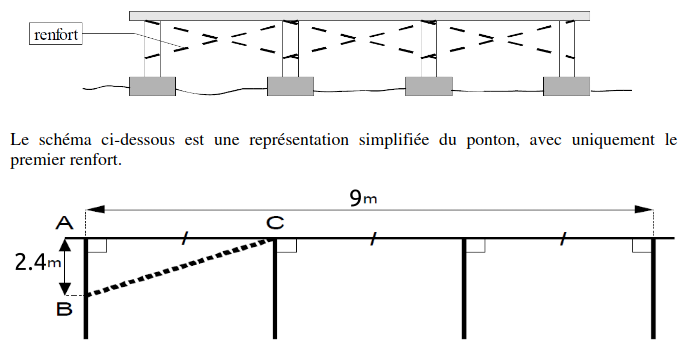
\includegraphics[width=0.6\linewidth]{4x7-pythagore-1/pb4a.png}
\end{figure}

\newpage


\textbf{DM - Pythagore}\\


\begin{center}
  \textit{Si nous faisions tout ce dont nous sommes capables, nous nous surprendrions vraiment.}  - \textbf{Thomas Edison}
\end{center}

\vspace{1cm} 

\subsubsection*{Pythagore Rédaction}

\begin{multicols}{2}
\begin{enumerate}
  \item[a.]Soit RTL un triangle rectangle en R tel que : RT = 37,5 cm et TL = 48,5 cm. \\
  \textbf{Calculer la longueur RL.}

  \item[b.]Soit LFD un triangle rectangle en D tel que : LF = 54,8 m et DL = 42 m. \\
  \textbf{Calculer la longueur FD.}

\end{enumerate}
\end{multicols}

\vspace{1cm} 

\subsubsection*{pb1.}

\begin{minipage}[t]{0.65\textwidth}
  Mario souhaite sauver la princesse Peach en haut d'un château haut de 45m. Pour cela, il jette un grappin par dessus les douves qui ont une longueur de 35m. Calculer la longueur nécessaire du grappin.

\vspace{1cm}
  
\end{minipage}
  \begin{minipage}[t]{0.35\textwidth}
  \begin{figure}[H]
    \centering
    \includegraphics[width=0.5\linewidth]{4x7-pythagore-1/pb1a.pdf}
  \end{figure}
\end{minipage}


\subsubsection*{pb2.} 

Mario doit grimper à l'échelle pour aller sauver la princesse. Pour être en sécurité une échelle de 8m doit être écarté de 2,5m du mur. À quelle hauteur maximale peut se trouver la princesse ? \\

\vspace{1cm}

\subsubsection*{pb3.}  

Mario doit traverser un pont mais celui-ci n'est pas assez solide. Il doit fixer 10 renforts en bois sur les poteaux verticaux qui soutiennent le ponton, comme le montre le dessin. Calculer la longueur d'un renfort puis calculer la longueur totale de tous les renforts nécessaires. 
  
\begin{figure}[H]
  \centering
  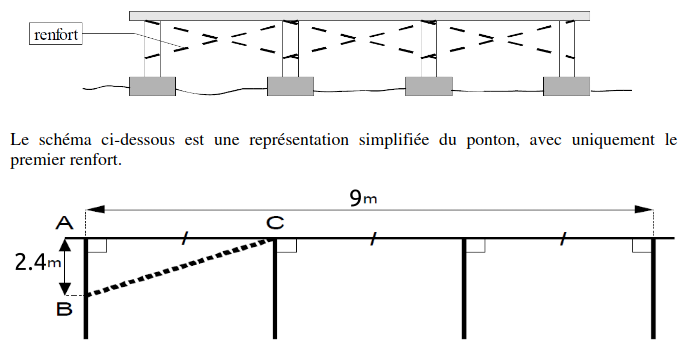
\includegraphics[width=0.6\linewidth]{4x7-pythagore-1/pb4a.png}
\end{figure}

\end{document}
